\subsection{Information entropy}
\label{exp:sec:entropy}

\begin{figure}[t]   
	\centering
	\begin{minipage}[t]{0.49\textwidth}
		\centering
		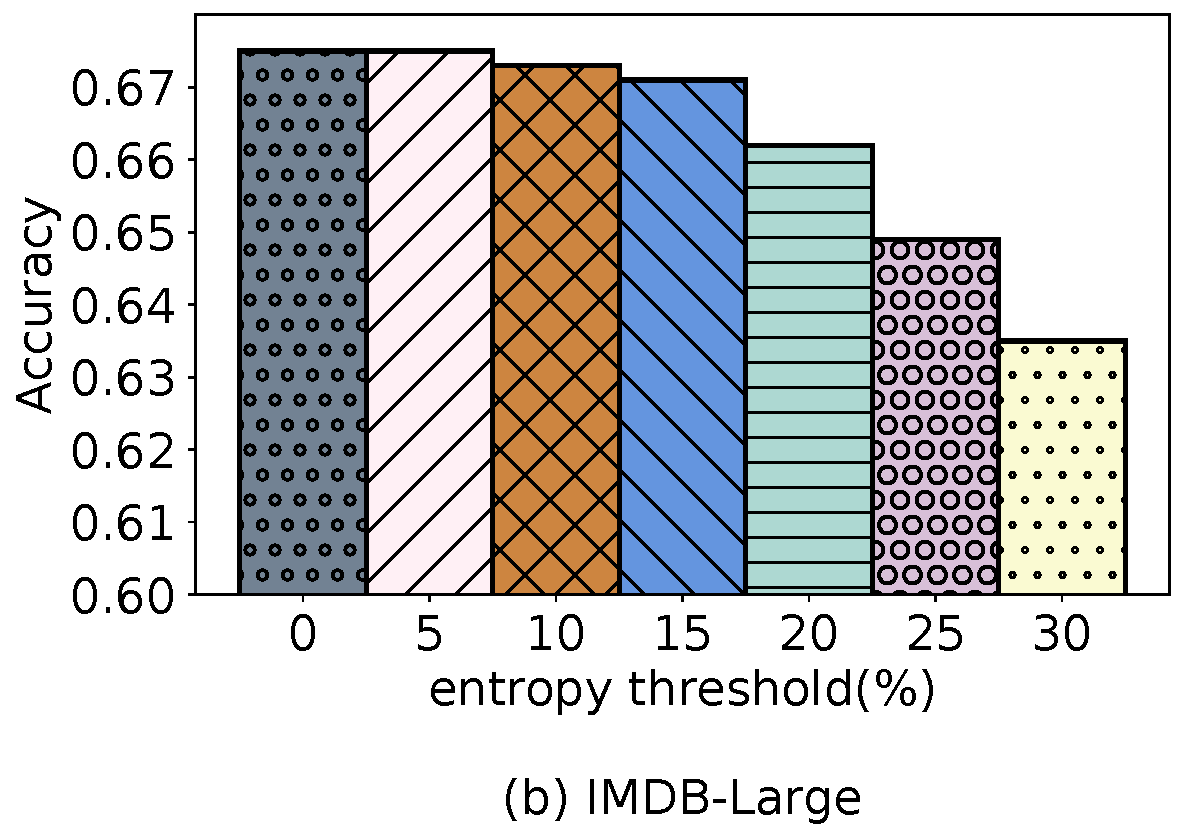
\includegraphics[width=\columnwidth]{figs/entropy_acc}
		\vspace{-1.5em}
		\caption{Effectiveness of \ours$^+$ for different Threshold.}
		\label{fig:entropy_acc}
	\end{minipage}
	\begin{minipage}[t]{0.49\textwidth}
		\centering
		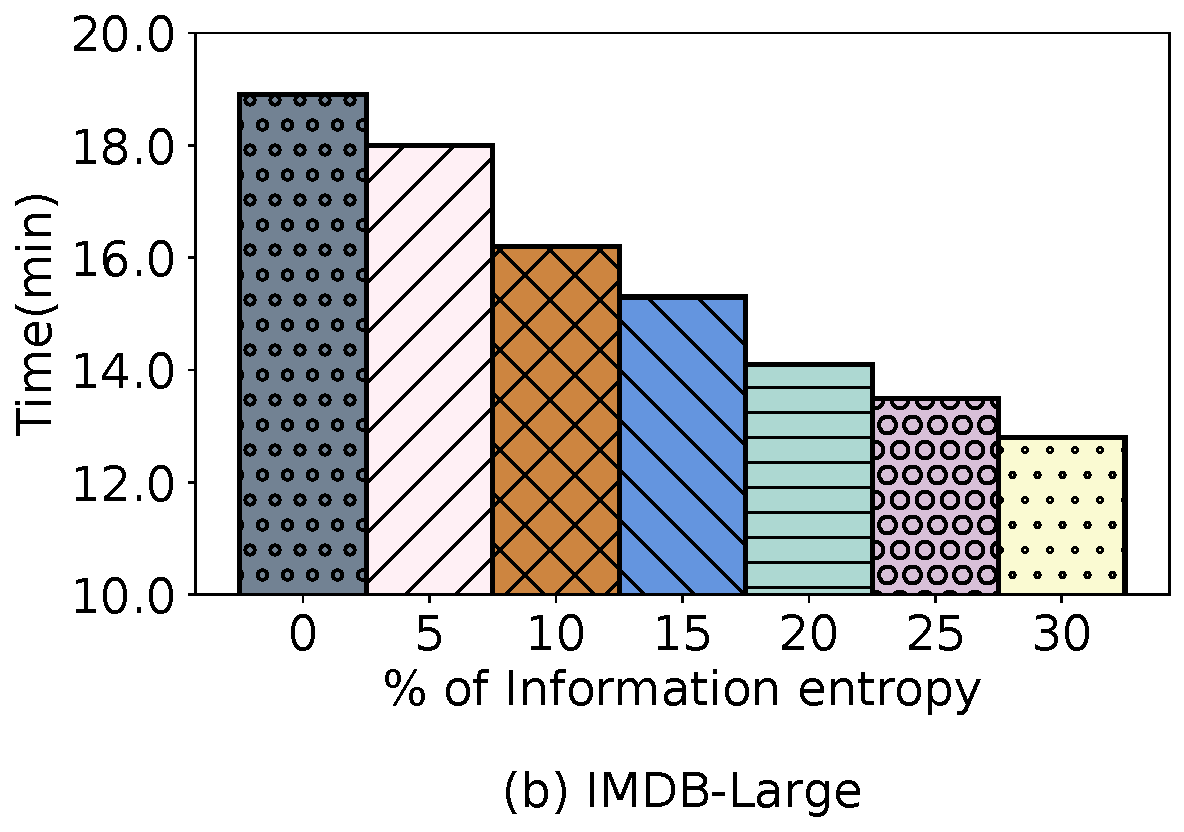
\includegraphics[width=\columnwidth]{figs/entropy_time}
		\vspace{-1.5em}
		\caption{Efficiency of \ours$^+$ for different Threshold.}
		\label{fig:entropy_time}
	\end{minipage}
	\vspace*{-1em}   
\end{figure}

In Section~\ref{subsec:clustering}, We use information entropy to preemptively fill in some missing values. In this part, we test the impact of different thresholds for the maximum information entropy. As shown in Figure~\ref{fig:entropy_acc}, when the threshold is below 15\%, the decrease in accuracy is not very significant. Conversely, when it exceeds 15\%, the rate of decrease accelerates. This is because when the threshold is low, all the candidate words filled in for the missing values have a high probability(\ie 90\%) and the threshold increases, the maximum probability gradually decreases, making the selection of candidate words for missing values more challenging. For example, on dataset \imdbl, when threshold is 15\%, the accuracy of \ours$^+$ is 71\%, which is only 0.4\% lower than when no processing is done at all.

Furthermore, we report the time change to reflect the efficiency of \ours$^+$ for different thresholds of information entropy. In Figure~\ref{fig:entropy_time}, we can see that the algorithm spends less and less time as the threshold increases because of the reduction in the number of incomplete tuples. On dataset \imdbl, when threshold is 30\%, the runtime of \ours$^+$ has decreased by over 30\%. And the runtime of \ours$^+$ decreased by approximately 3 minutes when threshold is 15\%.



In summary, we can use a appropriate threshold of information entropy to preemptively fill in some missing values, which can effectively reduce the runtime of \ours$^+$ while ensuring accuracy. 